% !TeX root = ../main.tex

\chapter{研究背景及意义}

传统的显著性目标检测是基于人工设计特征,但由于缺乏高级语义信息导致难以应用于复杂场景。伴随着机器学习的春风,显著性目标检测
也开始基于深度学习来提取显著性区域,并取得了不错的效果,如 PoolNet\cite{PoolNet},BASNet\cite{BASNet},AFNet\cite{AFNet}等。
由于能够模仿人类视觉找到显著性物体,显著性目标检测在计算机视觉方面发挥着重大作用,
显著性目标检测可以用于视频压缩编码:对图像的非显著区域设置较高的压缩比率,对图像的显著区域设置较低的压缩比率,这种模拟人类的视觉注意
来设置视频图像的压缩比率,具有广泛的适用性。此外,还可以应用于医学影像诊断,机器人避障等。

FFmpeg作为先进的跨平台的开源视频处理软件,能够完成视频封装与解封装,编码,解码,格式转换,本地播放,在线播放等功能,
除此之外,FFmpeg还有非常强大的滤镜功能,能够在后期对音视频进行多种多样的编辑。可谓是当代音视频处理领域的集大成者。
windows 上的 MPC(media player classic),Linux 平台上 MPlayer,以及以跨平台著称的后起之秀VLC,这三种多媒体播放框架均是基于FFmpeg。

尽管FFmpeg功能十分强大,但其中缺少对基于神经网络的图像处理算法的支持。我在知乎上\footnote{https://zhuanlan.zhihu.com/p/106192748}
看到刘歧前辈\footnote{FFmpeg 官方源代码维护者,资深音视频技术专家}曾经指导学生做过基于神经网络实现对图像进行去雨点、去雾的功能,并最终将其
加入了FFmpeg。本文以此为出发点,旨在探究在FFmpeg中嵌入基于神经网络的图像处理算法的方式,并提出了一种简单可行的方案。

首先,FFmpeg源码文件工程量巨大,使用configure脚本进行管理,而且单次编译耗时较久。倘若直接在源码中修改,那么每次测试时都需要重新编译
整个目录,效率非常低。为了解决这个问题,我的方案是先正常安装FFmpeg,然后把神经网络模型集成到播放器源码ffplay.c中,单独编译修改后的ffplay.c时,
只需要链接FFmpeg的动态库以及头文件,这可以使用CMake进行管理。工程的整体结构如图 \ref{fig:myplay} 所示,具体工程的创建步骤和细节在本文的第四章有详细介绍。
在这种方式下,每次编译测试仅需数秒的时间。

\begin{figure}[h]
\centering
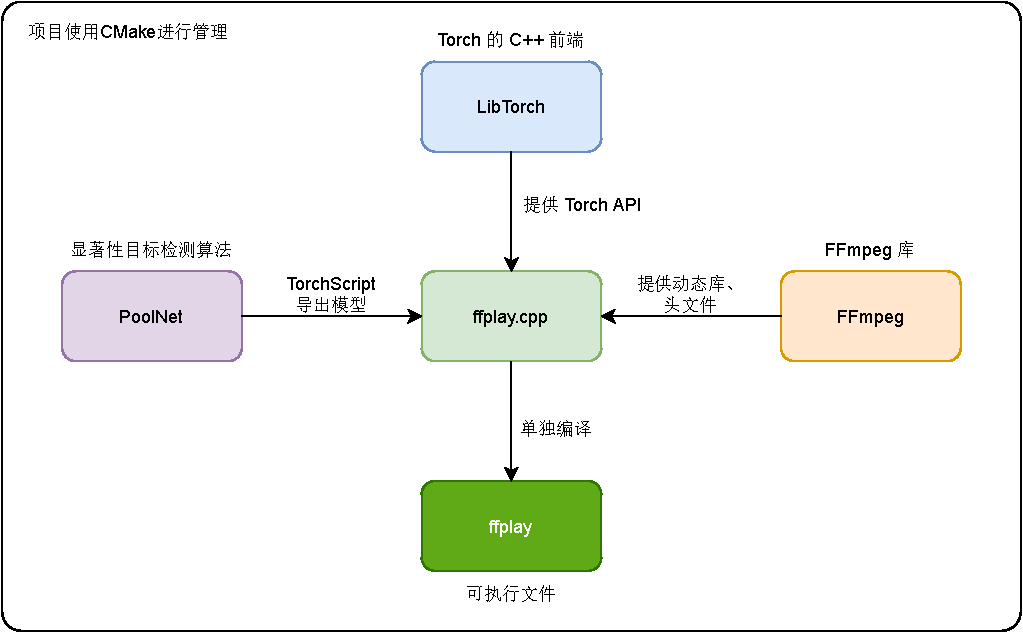
\includegraphics[width=1\textwidth]{myplay.pdf}
\caption{工程整体结构}
\label{fig:myplay}
% \note{注:图注的内容不宜放到图题中。}
\end{figure}

其次,嵌入的神经网络模型来自于PyTorch。当下机器学习的主流框架是TensorFlow和PyTorch,前者由谷歌开发,2015年发布,后者由FaceBook开发,
2017年发布。PyTorch虽然发布时间较晚,但因其简洁和易于使用的特点,目前已经和TensorFlow平分秋色。PyTorch提供了TorchScript工具,用于将神经网络
模型部署到生产环境中。除此之外,PyTorch还提供了C++前端的API,称之为LibTorch,以支持开发者在C++环境下搭建神经网络。

在实验中,我尝试了两种调用神经网络的方式:
一是使用TorchScript工具将模型导出,在C++前端直接调用模型;
二是使用LibTorch将神经网络重新构建为类对象,在C++前端把类对象实例化。
我在第五章结果与总结中对比了两种方法的效果。
总体来说,实验结果差强人意,对于输入为256x256的图片,在单个GeForce GTX 1080 Ti上运行时可以达到12fps。
